\documentclass{article}
\usepackage{tikz}
\usetikzlibrary{positioning}

\begin{document}

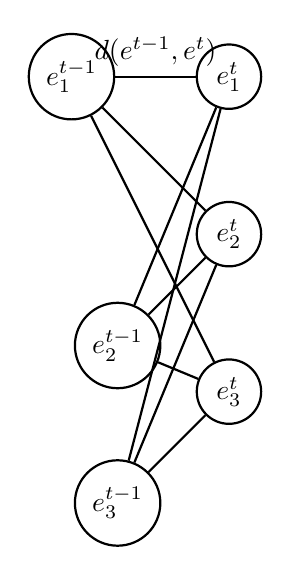
\begin{tikzpicture}[node distance={20mm}, thick, main/.style = {draw, circle}]
    \node[main] (1) {$e_1^{t}$};
    \node[main] (2) [below of=1] {$e_2^{t}$};
    \node[main] (3) [below of=2] {$e_3^{t}$};

    \node[main] (11) [left of=1] {$e_1^{t-1}$};
    \node[main] (21) [below left of=2] {$e_2^{t-1}$};
    \node[main] (31) [below left of=3] {$e_3^{t-1}$};

    \draw (1) -- node [above] {$d(e^{t-1}, e^{t})$} (11);
    \draw (1) -- (21);
    \draw (1) -- (31);
    \draw (2) -- (11);
    \draw (2) -- (21);
    \draw (2) -- (31);
    \draw (3) -- (11);
    \draw (3) -- (21);
    \draw (3) -- (31);
\end{tikzpicture}

\end{document}